\begin{figure}[htbp]
\centering
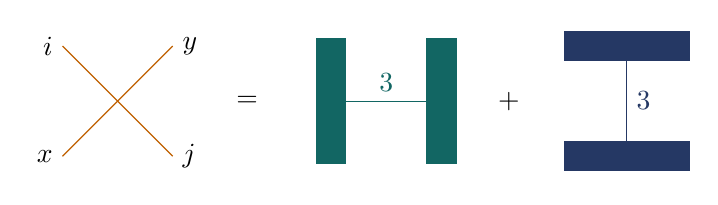
\begin{tikzpicture}[x=.7cm,y=.7cm]
  \definecolor{vertical}{RGB}{18,102,99}
  \definecolor{horizontal}{RGB}{37,56,100}
  \draw[orange!75!black] (0,0) node[left,text=black] {$x$} --
    (2,2) node[right,text=black] {$y$};
  \draw[orange!75!black] (0,2) node[left,text=black] {$i$} --
    (2,0) node[right,text=black] {$j$};
  \node at (3.35,1) {$=$};
  \foreach \x in {4.6,6.6}
    \fill[vertical] (\x,-.14) rectangle ++(.55,2.28);
  \draw[vertical] (5.15,1) -- (6.6,1) node[midway,above] {$3$};
  \node at (8.1,1) {$+$};
  \foreach \y in {-.27,1.73}
    \fill[horizontal] (9.1,\y) rectangle ++(2.28,.55);
  \draw[horizontal] (10.24,.28) -- (10.24,1.73) node[midway,right] {$3$};
\end{tikzpicture}
\caption{Two terms for a packet (numbers in bits). For either term one of the two ways of grouping
costs three, the other at most six, before adding selectors. One grouping will be chosen globally
using selector histograms.}
\label{fig:packet}
\end{figure}
